% Massimo Zannoni - Curriculum Vitae
%
% This work is licensed under a Creative Commons Attribution-ShareAlike 4.0 International License (CC BY-SA 4.0)

\documentclass[a4paper]{article}
\usepackage{graphicx}
\usepackage[top=2.4cm, bottom=2.4cm, left=2cm, right=2cm]{geometry}
\usepackage[utf8]{inputenc}
\usepackage{hyperref}
\usepackage[english]{babel}

%% set the font family
\usepackage[condensed,math]{kurier}
%% set the font encoding
\usepackage[T1]{fontenc}
%% details about the font
%% https://ctan.org/tex-archive/fonts/kurier/

%\usepackage{mdwlist} % needed for itemize*
%\usepackage{tabu} % package for advanced table features
\usepackage{longtable}
\usepackage{array}

\usepackage{enumitem}
%next line to avoid vertical separation before an itemize section
%\setlist{nolistsep}

% Personal details
\def\name{Name Surname}
\def\email{yourmail@goeshere.com}
\def\telephone{+00 11 22 33 44}
\def\nationality{Italian}
\def\dateofbirth{31.12.2020}
\def\gender{he\,/\,his}
\def\address{Mystreet, 1 \newline 0123 MyCity \newline MyCountry}

% Web links and logos
\def\githublink{https://github.com}
\def\gitlablink{https://gitlab.com}
\def\linkedinlink{https://linkedin.com}
% Official logos are not included in the repo, they can be found at the following links:
% GitHub: https://github.com/logos
\def\githublogo{pics/github-mark/github-mark.png}
% GitLab: https://about.gitlab.com/press/press-kit/#logos-rgb
\def\gitlablogo{pics/gitlab-logo/gitlab-logo-600.png}
% LinkedIn: https://brand.linkedin.com/downloads (black version created according to LinkedIn Logo Guidelines)
\def\linkedinlogo{pics/linkedin-logo/LI-In-Bug-black.png}

% Define some lengths used in the document
\newlength{\sectsep}
\setlength{\sectsep}{0.6cm}
\newlength{\subsectsep}
\setlength{\subsectsep}{0.4cm}
\newlength{\detsep}
\setlength{\detsep}{0.4cm}

% Edit PDF file properties
\hypersetup{
  pdfauthor = {\name},
  pdfcreator = {\name},
  pdfkeywords = {personal_skill_01, personal_skill_02, personal_interest_01, etc},
  pdftitle = {\name ~- Curriculum Vitae},
  pdfsubject = {Curriculum Vitae},
  % next line to avoid links from being blue and underlined
  hidelinks
}

% Format two pieces of text, one left aligned and one right aligned
\newcommand{\headerrow}[2]
{\begin{tabular*}{\textwidth}{l@{\extracolsep{\fill}}r}
	#1 &
	#2 \\
\end{tabular*}}

% Make lists with diamonds and compact spacing
\renewenvironment{itemize}{
  \begin{list}{$\diamond$}{
    \setlength{\topsep}{0.25em}
    \setlength{\itemsep}{0em}
    \setlength{\parskip}{0pt}
    \setlength{\parsep}{0em}
  }
}{
  \end{list}
}

% Make lists with small dots and compact spacing
\newenvironment{itemize2}{
  \begin{list}{$\cdot$}{
    \setlength{\topsep}{0.25em}
    \setlength{\itemsep}{0em}
    \setlength{\parskip}{0pt}
    \setlength{\parsep}{0em}
  }
}{
  \end{list}
}

\begin{document}
  \begin{longtable}{r || l}

  % 1st row: Title, details and photo
  \hfill
  & \begin{minipage}{0.5\textwidth}
      \vspace{0.2\sectsep}
      \section*{\name}
      \vspace{\detsep}
      \address \vspace{\detsep} \\
      \href{mailto:\email}{\email} ~|~ \telephone \vspace{\detsep} \\
      \dateofbirth ~|~ \nationality ~|~ \gender \vspace{\detsep} \\
    \end{minipage}
    %\hfill
    \begin{minipage}{0.3\textwidth}
      \vspace{0.4cm}
      {\centering
      	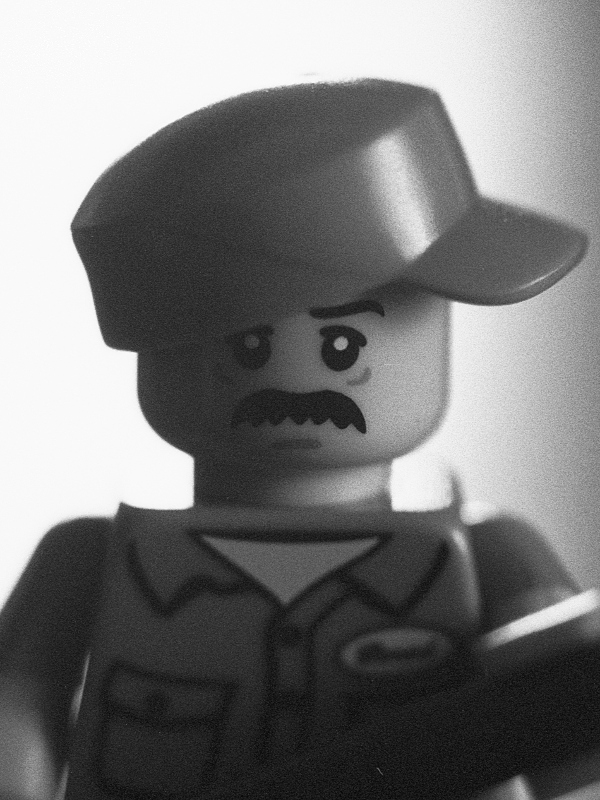
\includegraphics[width=0.5\textwidth]{pics/portrait} \vspace{0.1cm} \\
      	% raisebox is used to center the logos vertically
        \raisebox{-0.5\height}{\href{\githublink}{\includegraphics[height=3.2ex]{\githublogo}}}
        ~
        \raisebox{-0.5\height}{\href{\gitlablink}{\includegraphics[height=4ex]{\gitlablogo}}}
        ~
        \raisebox{-0.5\height}{\href{\linkedinlink}{\includegraphics[height=3.2ex]{\linkedinlogo}}}
        \vspace{0.1cm}
      \\
      }
    \end{minipage} \\
  \hline \hline

  %2nd row: Working experience 1
  & \begin{minipage}{0.9\textwidth}
      \vspace{\sectsep}
      \subsection*{Working Experience}
      \subsubsection*{Position X}
      \headerrow
  		{\textbf{Company X}}{\emph{2056 - current}}
      \\
      \headerrow
        {\emph{Address X, 0001 CityX, StateX}}{}
      \\
      \headerrow
        {Field of Company X}{}

      \begin{itemize}
          \item Activity 1
          \begin{itemize2}
              \item Further specify Activity 1
          \end{itemize2}
          \item Activity 2
          \item Key Responsibility 1
          \item Key Responsibility 2
      \end{itemize}
  \end{minipage} \\[\sectsep]

  %3rd row: Working experience 2
  & \begin{minipage}{0.9\textwidth}
      \vspace{\subsectsep}
      \subsubsection*{Position Y}
      \headerrow
  		{\textbf{Company Y}}{\emph{2050 - 2056}}
      \\
      \headerrow
        {\emph{Address Y, 0002 CityY, StateY}}{}
      \\
      \headerrow
          {Field of Company Y}{}

      \begin{itemize}
          \item Activity 1
          \item Activity 2
      \end{itemize}
  \end{minipage} \\[\sectsep]

  %4th row: Working experience 3
  % & \begin{minipage}{0.9\textwidth}
  %     \vspace{\sectsep}
    %   \subsubsection*{Position Z}
    %   \headerrow
 %  		{\textbf{Company Z}}{\emph{2045 - 2050}}
    %   \\
    %   \headerrow
    %     {\emph{Address Z, 0003 City Z, StateZ}}{}
    %   \\
    %   \headerrow
    %       {Field of Company Z}{}
    %
    % %   \begin{itemize}
    % %       \item Key Responsibility 1
    % %       \item Key Responsibility 2
    % %   \end{itemize}
  % \end{minipage} \\[\sectsep]

  %5th row: Education 1
  & \begin{minipage}{0.9\textwidth}
      \vspace{\sectsep}
      \subsection*{Education}
      \subsubsection*{MSc in This Discipline}
      \headerrow
  		{\textbf{University X}}{\emph{2043 - 2045}}
      \\
      \headerrow
        {\emph{Faculty of This Discipline}}{}
      \\
      \headerrow
        {Field of Study 1, Field of Study 2}{}

      \begin{itemize}
          \item Thesis: \emph{Something really difficult}
          \item Grade: x/y
      \end{itemize}
  \end{minipage} \\[\sectsep]

  %6th row: Education 2
  & \begin{minipage}{0.9\textwidth}
      \vspace{\subsectsep}
      \subsubsection*{BSc in That Discipline}
      \headerrow
  		{\textbf{University Y}}{\emph{2040 - 2043}}
      \\
      \headerrow
        {\emph{Faculty of That Discipline}}{}
      \\
      \headerrow
        {Field of Study 1, Field of Study 2}{}

      \begin{itemize}
          \item Thesis: \emph{Something quite easy}
          \item Grade: x/y
      \end{itemize}
      \vfill
  \end{minipage} \\[\sectsep]

  %7th row: Personal skills and competences
  & \begin{minipage}{0.9\textwidth}
      \vspace{\sectsep}
      \subsection*{Skills and Competences}
      \subsubsection*{Languages}
      \begin{tabular}{rl}
        \textbf{Italian:}&Native\\
        \textbf{English:}&Fluent\\
        \textbf{German:}&Beginner/Intermediate\\
      \end{tabular} \vspace{1.5ex} \\
      %\hspace*{0.5em} {\footnotesize \emph{See Common European Framework (CEF) self-assessment table in the appendix.}}
    \end{minipage} \\[\sectsep]

  %8th row: Technical skills and competences
  & \begin{minipage}{0.9\textwidth}
      \vspace{\subsectsep}
      \subsubsection*{Technical and Organizational}
      \begin{itemize}
          \item Technical Skill X
          \item Social Competence Y
          \item Managerial Skill Z
          \item Special Competence W
      \end{itemize}
  \end{minipage} \\[\sectsep]

  %9th row: Computer skills and competences
  & \begin{minipage}{0.9\textwidth}
      \vspace{\subsectsep}
      \subsubsection*{Computer Tools and Software Development}
      \begin{tabular*}{\textwidth}{r p{0.75\textwidth}}
        Operating Systems:&{Linux: very good knowledge\newline Microsoft Windows: good knowledge}\\[0.5ex]
        Electronic CAD:&Cadence DFII (Virtuoso, Spectre), SPICE, Cadence OrCAD (PSpice), Cadence SoC Encounter, Agilent ADS\\[0.5ex]
        Programming:&Python, C/C++, Matlab/Octave, shell scripting, VHDL, Verilog/VerilogA, {\fontfamily{cmr}\selectfont\LaTeX}\\[0.5ex]
        Version Control:&Subversion, Git
      \end{tabular*}\\
  \end{minipage} \\[\sectsep]

  %10th row: Other skills and competences
  & \begin{minipage}{0.9\textwidth}
      \vspace{\subsectsep}
      \subsubsection*{Others}
      \begin{itemize}
          \item Amateur Skill 1
          \item Hobby Competence 2
          \item Driving License: Category X
      \end{itemize}
  \end{minipage} \\[\sectsep]

  %11th row: Personal Interests
  & \begin{minipage}{0.9\textwidth}
      \vspace{\subsectsep}
      \subsubsection*{Personal Interests}
      \begin{itemize}
          \item Blue skies
          \item Sweet fruits
      \end{itemize}
  \end{minipage} \\[\sectsep]

  %12th row: Annexes
  & \begin{minipage}{0.9\textwidth}
      \vspace{\subsectsep}
      \subsubsection*{Annexes}
      \begin{itemize}
          \item Appendix including some more boring specs
          \item Reference letter by Mr He
      \end{itemize}
      \vfill
    \end{minipage} \\

  \end{longtable}
\end{document}
